In this chapter we will show how we have implemented the architectures presented in chapter \ref{chapter:architectures}.

\section{Testing Program}
We have developed two applications in Emerald to test computation offloading and storage offloading. Each of them are easily configurable and flexible for testing. The next two subsections will show how they are implemented.

\subsection{Computation offloading}
For computation offloading we initially wanted to implement Eratosthenes Sieve for finding primes. This is because it has an interesting way parallelizing, and therefore distributing the work. However, due to an limitation from the Emerald VM, memory runs out when trying to find relatively low primes. This can be optimized, but it does not change the fact that Eratosthenes Sieve is a memory intensive application. Therefore we are doing hashing instead. Hashing is a low memory, compute intensive task. This is excellent for our simulation as we primarily want to focus on computational use and latency.

\subsection{Hashing algorithm}
The hashing algorithm we use is called \textit{Djb2}. Our implementation is a converted version from a C implementation found here\cite{noauthor_hash_nodate}.
\begin{lstlisting}[language=emerald]
function djb2Hash[str: String] -> [res: Integer]
  res <- 5381
  for i : Integer <- 0 while i < str.length 
                                    by i <- i + 1
    res <- res * 33 * str[i].ord
  end for
end djb2Hash
\end{lstlisting}
The algorithm takes a string, iterates over it and multiplies itself with 33 and the characters ordinal number. To make it even heavier, we convert the result to string, and then re-insert that into the hash function 10000 times. We see that as one iteration, as shown in figure \ref{fig:Hashing_algorithm_iteration}. In other words, the HashWorker will do what figure \ref{fig:Hashing_algorithm_iteration} shows, parameter \verb|iterations| number of times. Since we just throw out the result after each time, Emeralds garbage compiler will ensure that we have plenty of memory available. 
\begin{figure}[t]
    \centering
    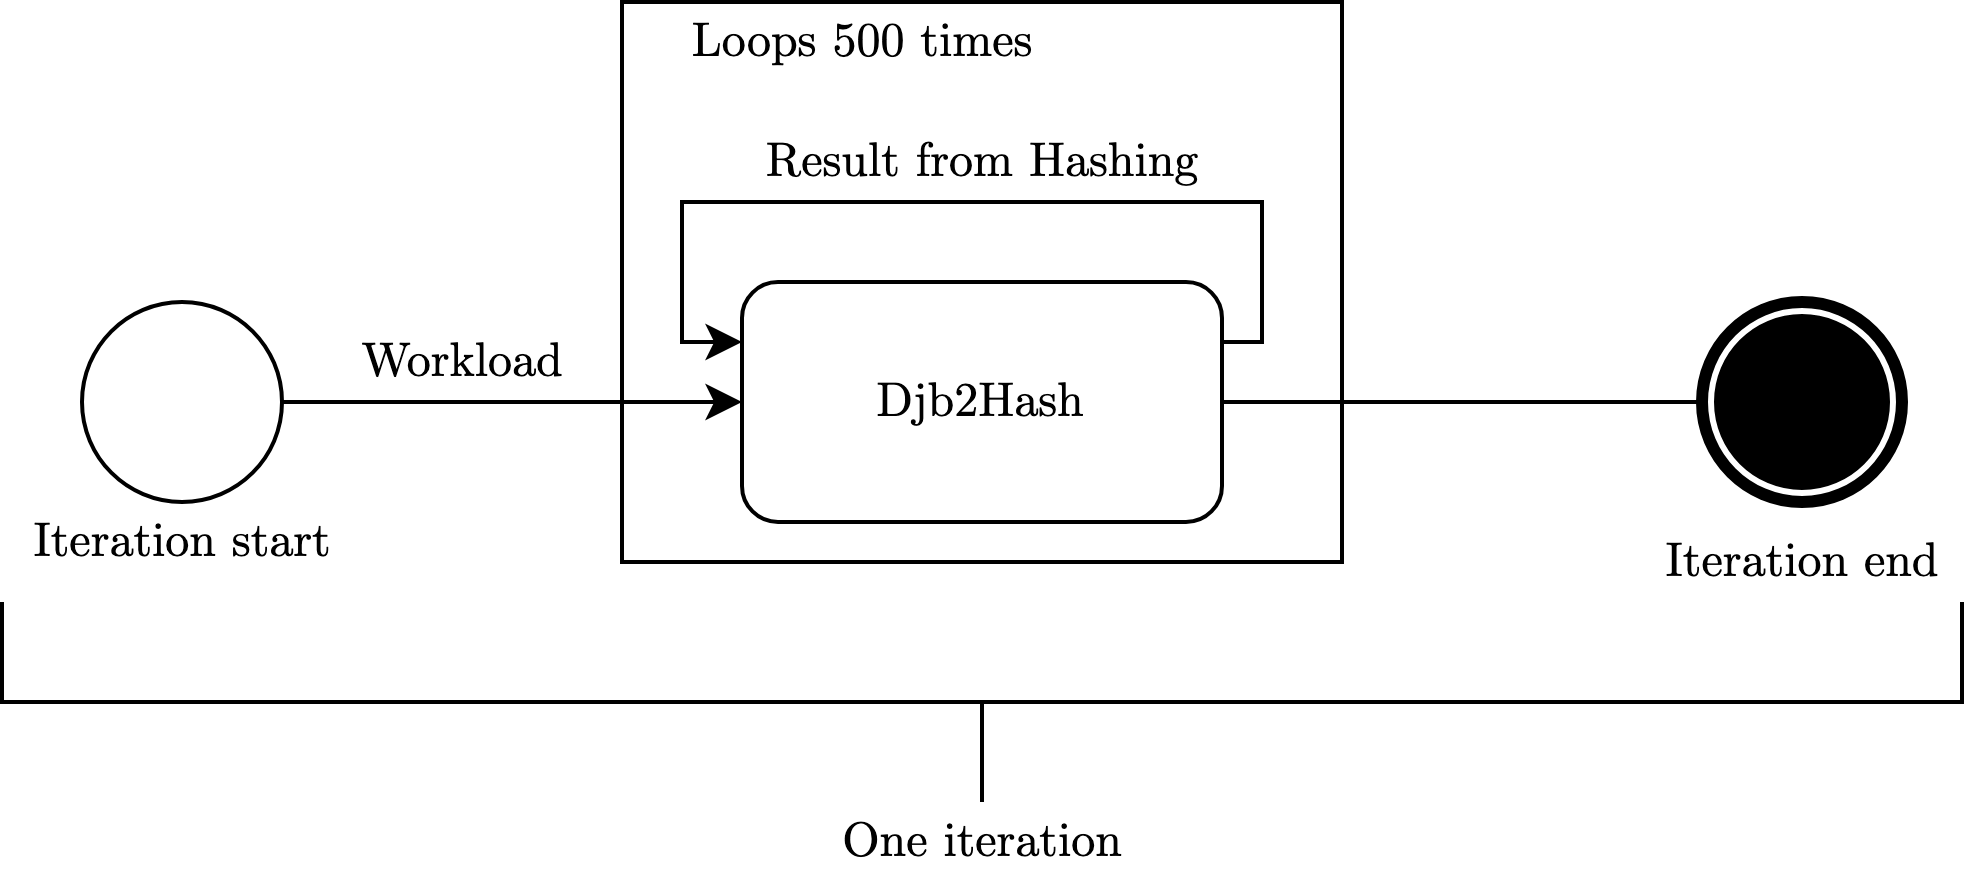
\includegraphics[scale=0.9]{chapters/implementation/figures/Iteration.png}
    \caption{Illustration of one iteration in the HashWorker}
    \label{fig:Hashing_algorithm_iteration}
\end{figure}




\subsection{Classes and structure}
Figure TODO illustrates how two nodes will be set up. Blablabla.


\subsection{Simulating CPU restrictions}
To simulate CPU restrictions, we place a limitation on each HashWorker. This limitation is implemented as time delay. For each iteration a time delay is called. The amount of microseconds delayed is the \verb|limitation| parameter multiplied by 1000. 

\subsection{Storage offloading}


\section{Multi-Access Edge Computing}
TODO
% Vis de forskjellige måtene og ta storage offloading på


\subsection{Limitation}
Originally we wanted to use monitors. However when there is a case in Emerald where if you have to separate objects containing each of their own monitor with condition. Then when waiting on these separate conditions just exits the program when hitting the other condition!

